\documentclass[12pt,oneside,a4paper]{book}

%\usepackage[utf8]{inputenc}
%\usepackage[T1]{fontenc}
\usepackage[english]{babel}

\usepackage{amsmath}
\usepackage{amssymb}
\usepackage{amsthm}
\usepackage{graphics}
\usepackage{enumerate}
\usepackage{amscd}
\usepackage{tikz}
\usetikzlibrary{shapes}

%%%% Layout %%%%%%%%%%%%%%%%%
\addtolength{\evensidemargin}{-2cm}
\addtolength{\oddsidemargin}{-2cm}
\setlength{\textwidth}{17cm} 
\setlength{\textheight}{26.5cm} 
\addtolength{\topmargin}{-3cm}
\setlength{\parindent}{0pt}
\pagestyle{plain}

\newcounter{probnum}
\newcounter{solnum}
\setcounter{probnum}{0}
\newcommand{\prob}{\ifnum\value{probnum}>0\newpage\fi\setcounter{solnum}{0}\stepcounter{probnum}\textbf{Problem \theprobnum}\\}
\newcommand{\ans}{\medskip\hrule\medbreak\emph{Answer: }}
\newcommand{\comment}{\medskip\hrule\medbreak\emph{Comment: }}
\newcommand{\sol}{\medskip\hrule\medbreak\textbf{Solution}\\}
\newcommand{\soln}{\stepcounter{solnum}\medskip\hrule\medbreak\textbf{Solution \thesolnum}\\}
\newcommand{\marking}{\medskip\hrule\medbreak\textbf{Marking scheme -- Problem \theprobnum}}

\newcommand*\circled[1]{\tikz[baseline=(char.base)]{
            \node[shape=circle,draw,inner sep=2pt] (char) {#1};}}

\newcommand{\s}{\phantom{s}}

\begin{document}
\begin{center}
\textbf{\large APMO 1993 -- Problems and Solutions}
\end{center}

% Problem 1
\prob Let $ABCD$ be a quadrilateral such that all sides have equal length and angle $\angle ABC$ is 60 degrees.  Let $\ell$ be a line passing through $D$ and not intersecting the quadrilateral (except at $D$). Let $E$ and $F$ be the points of intersection of $\ell$ with $AB$ and $BC$ respectively. Let $M$ be the point of intersection of $CE$ and $AF$.

Prove that $CA^2=CM\times CE$.

\sol
\begin{center}
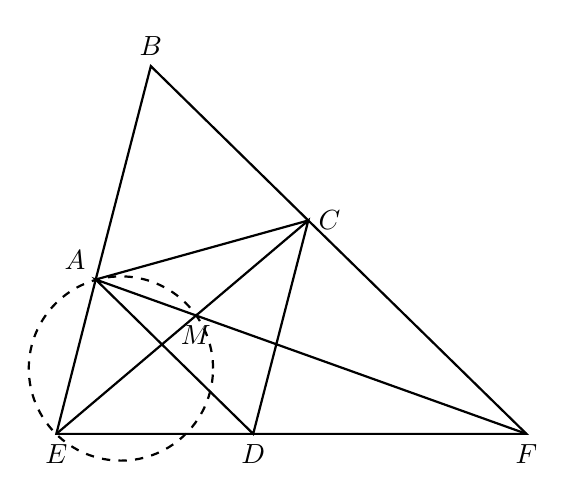
\begin{tikzpicture}
\draw[thick] (2.48,2.94) node[anchor=south] {$B$} -- (1.78,0.23) node[anchor=south east] {$A$} -- (1.28,-1.73) node[anchor=north] {$E$} -- (3.78,-1.73) node[anchor=north] {$D$} -- (7.25,-1.73) node[anchor=north] {$F$} -- (4.48,0.98) node[anchor=west] {$C$} -- cycle;
\draw[thick] (1.28,-1.73) -- (4.48,0.98) -- (3.78,-1.73) -- (1.78,0.23) -- (7.25,-1.73);
\draw[thick] (1.78,0.23) -- (4.48,0.98);
\draw (3.05,-0.23) node[anchor=north] {$M$};
\draw[thick,dashed] (2.1,-0.9) circle (1.17);
\end{tikzpicture}
\end{center}

Triangles $AED$ and $CDF$ are similar, because $AD\parallel CF$ and $AE\parallel CD$. Thus, since $ABC$ and $ACD$ are equilateral triangles,
\[\frac{AE}{CD} = \frac{AD}{CF}\iff \frac{AE}{AC} = \frac{AC}{CF}.\]

The last equality combined with
\[\angle EAC = 180^\circ - \angle BAC = 120^\circ = \angle ACF\]
shows that triangles $EAC$ and $ACF$ are also similar. Therefore $\angle CAM = \angle CAF = \angle AEC$, which implies that line $AC$ is tangent to the circumcircle of $AME$. By the power of a point, $CA^2 = CM\cdot CE$, and we are done.

% Problem 2
\prob Find the total number of different integer values the function
\[f(x)=[x]+[2x]+\left[\frac{5x}3\right]+[3x]+[4x]\]
takes for real numbers $x$ with $0\le x\le 100$.

\emph{Note:} $[t]$ is the largest integer that does not exceed $t$.

\ans $734$.

\sol
Note that, since $[x+n] = [x]+n$ for any integer $n$,
\[f(x+3) = [x+3] + [2(x+3)] + \left[\frac{5(x+3)}3\right] + [3(x+3)] + [4(x+3)] = f(x) + 35,\]
one only needs to investigate the interval $[0,3)$.

The numbers in this interval at which at least one of the real numbers $x,2x,\frac{5x}3,3x,4x$ is an integer are
\begin{itemize}
\item $0,1,2$ for $x$;
\item $\frac n2$, $0\le n\le 5$ for $2x$;
\item $\frac{3n}5$, $0\le n\le 4$ for $\frac{5x}3$;
\item $\frac n3$, $0\le n\le 8$ for $3x$;
\item $\frac n4$, $0\le n\le 11$ for $4x$.
\end{itemize}

Of these numbers there are
\begin{itemize}
\item $3$ integers ($0,1,2$);
\item $3$ irreducible fractions with $2$ as denominator (the numerators are $1,3,5$);
\item $6$ irreducible fractions with $3$ as denominator (the numerators are $1,2,4,5,7,8$);
\item $6$ irreducible fractions with $4$ as denominator (the numerators are $1,3,5,7,9,11,13,15$);
\item $4$ irreducible fractions with $5$ as denominator (the numerators are $3,6,9,12$).
\end{itemize}

Therefore $f(x)$ changes values $22$ per interval. Since $100 = 33\cdot 3 + 1$, there are $33\cdot 22$ changes in $[0,99)$. Finally, there are $8$ more changes in $[99,100]$: $99$, $100$, $99\frac12$, $99\frac13$, $99\frac23$, $99\frac14$, $99\frac34$, $99\frac35$.

The total is then $33\cdot 22+8=734$.

\comment
A more careful inspection shows that the range of $f$ are the numbers congruent modulo $35$ to one of
\[0, 1, 2, 4, 5, 6, 7, 11, 12, 13, 14, 16, 17, 18, 19, 23, 24, 25, 26, 28, 29, 30\]
in the interval $[0,f(100)] = [0,1166]$. Since $1166 \equiv 11\pmod{35}$, this comprises $33$ cycles plus the $8$ numbers in the previous list.

% Problem 3
\prob Let
\[f(x) = a_nx^n+a_{n-1}x^{n-1}+\cdots+a_0\quad\text{and}\quad g(x)=c_{n+1}x^{n+1}+c_nx^n+\cdots+c_0\]
be non-zero polynomials with real coefficients such that $g(x)=(x+r)f(x)$ for some real number $r$. If $a=\max(|a_n|,\ldots,|a_0|)$ and $c=\max(|c_{n+1}|,\ldots,|c_0|)$, prove that $\frac ac \le n+1$.

\sol
Expanding $(x+r)f(x)$, we find that $c_{n+1} = a_n$, $c_k=a_{k-1}+ra_k$ for $k=1,2,\ldots,n$, and $c_0=ra_0$.

Consider three cases:
\begin{itemize}
\item $r=0$. Then $c_0=0$ and $c_k = a_{k-1}$ for $k=1,2,\ldots,n$, and $a=c\implies \frac ac=1<n+1$.
\item $|r|\ge 1$. Then
\begin{gather*}
|a_0| = \left|\frac{c_0}r\right| \le c,\\
|a_1| = \left|\frac{c_1-a_0}r\right| \le |c_1|+|a_0| \le 2c,
\end{gather*}
and inductively if $|a_k| \le (k+1)c$
\[|a_{k+1}| = \left|\frac{c_{k+1}-a_k}r\right| \le |c_{k+1}| + |a_k| \le c+(k+1)c=(k+2)c.\]
Therefore, $|a_k| \le (k+1)c \le (n+1)c$ for all $k$, and $a \le (n+1)c\iff \frac ac\le n+1$.
\item $0 < |r| < 1$. Now work \emph{backwards}: $|a_n| = |c_{n+1}| \le c$,
\[|a_{n-1}| = |c_n - ra_n| \le |c_n| + |ra_n| < c + c = 2c,\]
and inductively if $|a_{n-k}| \le (k+1)c$
\[|a_{n-k-1}| = |c_{n-k} - ra_{n-k}| \le |c_{n-k}| + |ra_{n-k}| < c + (k+1)c = (k+2)c.\]
Therefore, $|a_{n-k}| \le (k+1)c \le (n+1)c$ for all $k$, and $a\le (n+1)c$ again.
\end{itemize}

% Problem 4
\prob Determine all positive integers $n$ for which the equation
\[x^n+(2+x)^n+(2-x)^n=0\]
has an integer as a solution.

\ans $n=1$.

\sol
If $n$ is even, $x^2+(2+x)^n+(2-x)^n > 0$, so $n$ is odd.

For $n=1$, the equation reduces to $x+(2+x)+(2-x)=0$, which has the unique solution $x=-4$.

For $n>1$, notice that $x$ is even, because $x$, $2-x$, and $2+x$ have all the same parity. Let $x=2y$, so the equation reduces to
\[y^n + (1+y)^n + (1-y)^n = 0.\]

Looking at this equation modulo $2$ yields that $y+(1+y)+(1-y)=y+2$ is even, so $y$ is even. Using the factorization
\[a^n + b^n = (a+b)(a^{n-1}-a^{n-2}b+\cdots+b^{n-1})\quad\text{for }n\text{ odd},\]
which has a sum of $n$ terms as the second factor, the equation is now equivalent to
\[y^n + (1+y+1-y)((1+y)^{n-1}-(1+y)^{n-2}(1-y) + \cdots +(1-y)^{n-1}) = 0,\]
or
\[y^n = -2((1+y)^{n-1}-(1+y)^{n-2}(1-y) + \cdots +(1-y)^{n-1}).\]

Each of the $n$ terms in the second factor is odd, and $n$ is odd, so the second factor is odd. Therefore, $y^n$ has only one factor $2$, which is a contradiction to the fact that, $y$ being even, $y^n$ has at least $n>1$ factors $2$. Hence there are no solutions if $n>1$.

% Problem 5
\prob Let $P_1,P_2,\ldots,P_{1993}=P_0$ be distinct points in the $xy$-plane with the following properties:
\begin{enumerate}[(i)]
\item both coordinates of $P_i$ are integers, for $i=1,2,\ldots,1993$;
\item there is no point other than $P_i$ and $P_{i+1}$ on the line segment joining $P_i$ with $P_{i+1}$ whose coordinates are both integers, for $i=0,1,\ldots,1992$.
\end{enumerate}

Prove that for some $i$, $0\le i\le 1992$, there exists a point $Q$ with coordinates $(q_x,q_y)$ on the line segment joining $P_i$ with $P_{i+1}$ such that both $2q_x$ and $2q_y$ are odd integers.

\sol
Call a point $(x,y)\in\mathbb{Z}^2$ \emph{even} or \emph{odd} according to the parity of $x+y$. Since there are an odd number of points, there are two points $P_i = (a,b)$ and $P_{i+1} = (c,d)$, $0\le i\le 1992$ with the same parity. This implies that $a+b+c+d$ is even. We claim that the midpoint of $P_iP_{i+1}$ is the desired point $Q$.

In fact, since $a+b+c+d=(a+c)+(b+d)$ is even, $a$ and $c$ have the same parity if and only if $b$ and $d$ also have the same parity. If both happen then the midpoint of $P_iP_{i+1}$, $Q=\left(\frac{a+c}2,\frac{b+d}2\right)$, has integer coordinates, which violates condition (ii). Then $a$ and $c$, as well as $b$ and $d$, have different parities, and $2q_x=a+c$ and $2q_y=b+d$ are both odd integers.

\end{document}